\chapter{Fundamentos Teóricos}
\section{Image Quality Assessment (IQA)}
\label{sec:IQA}
Existen tres subproblemas presenten en el ámbito de \emph{IQA}~\cite{RecentIQASurvey, IQABook, VisualMedicalQualityBook}. Los primeros, son problemas 
donde tenemos acceso a la imagen original, que suponemos exenta de desperfectos, 
en la cual se pueden aplicar métodos basados en diferencia de características 
entre ambas, como puede ser al nivel del color de píxel posición a posición,
y se denomina ``\emph{Full Reference}''(\emph{FR}). 
La tarea, aparentemente sencilla, en realidad presenta una complejidad alta dada por 
la necesidad de codificar la percepción humana a la hora de calificar la calidad 
de una imagen~\cite{WhyIsIQASoDifficult}, ya que métricas que miden distancias no suelen 
ser suficientes al no haber buena correlación entre la calidad percibida y el 
resultado de la métrica.

La mayoría de las veces no se menciona, pero al optar métodos de sensibilidad 
al error (distancias) se imponen un conjunto de suposiciones cuestionables. 
Primeramente, se asume la misma importancia para todas las señales de la imagen\footnote{
  Con \emph{señales} nos referimos a los diferentes canales de color RGB.
}, que
la magnitud del error es lo único que determina la calidad, que el contenido de la imagen 
no afecta al resultado final tras aplicar una distorsión, y que si cambiamos el 
orden de las señales la medida de distorsión no es afectada.
Lamentablemente, ninguna de estas suposiciones se cumplen~\cite{Wang2006ModernIQ} (véasen Figuras \ref{fig:FailureMinkowskiMetric} y \ref{fig:MSEHyperSphere}, 
que utilizan distancias \emph{Minkowski}, 
que puede considerarse como una generalización tanto de 
la distancia euclídea como de la distancia de Manhattan, 
y \emph{MSE}, 
que se calcula como la media de la suma de las 
diferencias al cuadrado, respectivamente).

\begin{figure}[htp]
  \begin{center}
    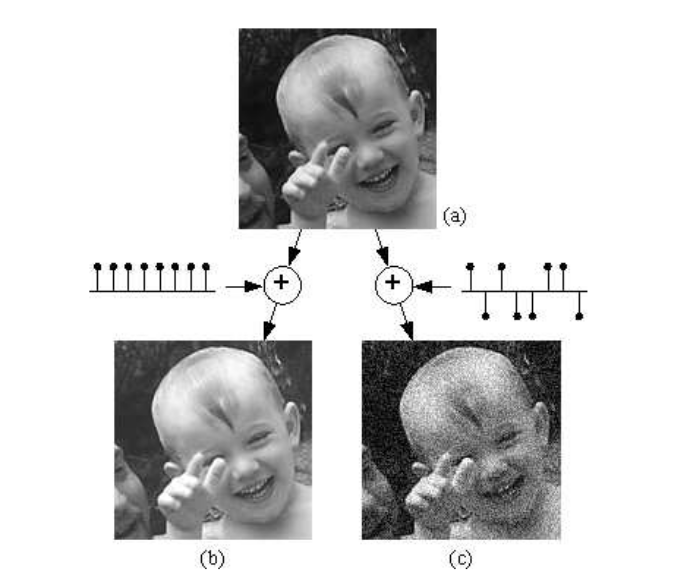
\includegraphics[width=0.6\textwidth]{imagenes/chapter2/failure_minkowski_metric.png}
  \end{center}
  \caption[Visualización del problema de la métrica \emph{Minkowski}.]{En este ejemplo, extraído de~\cite{MinkowskiFailure},
  vemos que sumar una constante positiva a una imagen  de referencia (a) produce la imagen (b) que contiene la misma distancia \emph{Minkowski}
  que (c), imagen fabricada por la misma constante pero permutando signo de forma aleatoria, resultando que
  la percepción final es que la imagen (c) es peor que la imagen (b).
\label{fig:FailureMinkowskiMetric}}
\end{figure}
\begin{figure}[htp]
  \begin{center}
    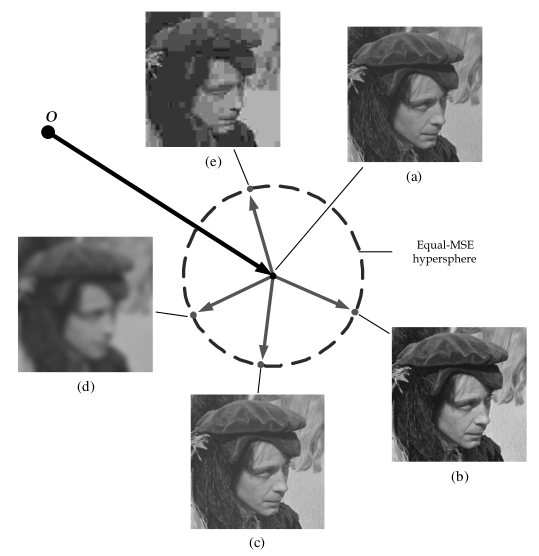
\includegraphics[width=0.6\textwidth]{imagenes/chapter2/MSE_Hypersphere.png}
  \end{center}
  \caption[Visualización del hiperplano MSE de imágenes distorsionadas.]{En este ejemplo, extraído de~\cite{Wang2006ModernIQ}, la misma imagen distorsionada de distintas 
    maneras resulta en la misma distancia, con valor MSE=181. 
    No obstante, es evidente que algunas distorsiones producen efectos visuales más marcados que otras.}
  \label{fig:MSEHyperSphere}
\end{figure}
 
El siguiente subproblema es aquel donde tenemos algún tipo de información adicional, incompleta, respecto 
a la imagen original el momento de análisis de la calidad de la imagen final,
denominados ``\emph{Reduced Reference}''(\emph{RR}). La información extra puede 
incluir metadatos, parámetros 
de compresión, características estadísticas o extraídas de una región de interés específica.
 
Y por último, tenemos aquellos problemas donde desconocemos el origen y cualquier 
información respecto a la imagen inicial, denominados problemas ``\emph{No reference}''(\emph{NR}).
Estas métricas están exentas de cualquier información de referencia y se 
centran en capturar características generales de calidad.

\begin{figure}[htp]
  \centering
  \begin{subfigure}{0.49\textwidth}
  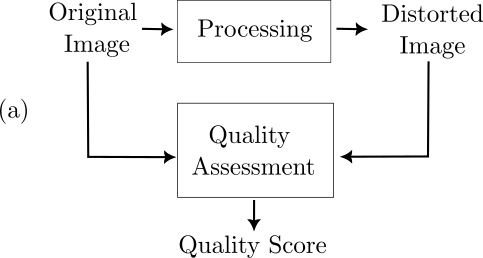
\includegraphics[width=0.95\textwidth]{imagenes/chapter2/FullReferenceInk.png}
  \end{subfigure}
  \begin{subfigure}{0.49\textwidth}
  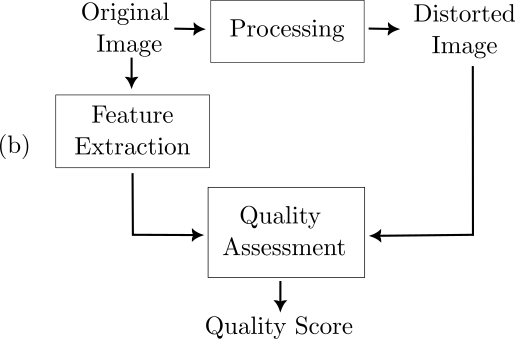
\includegraphics[width=0.95\textwidth]{imagenes/chapter2/ReducedReferenceInk.png}
  \end{subfigure}
  \par\bigskip
  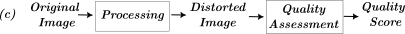
\includegraphics[]{imagenes/chapter2/NoReferenceInk.png}
  \caption{Resumen de subproblemas IQA. La imagen (a) representa el subproblema FR, 
  la imagen (b) RR y la imagen (c) NR.}
  \label{fig:IQASubproblems}
\end{figure}


La evaluación de calidad de imagen sin referencia es, quizás, el problema 
más difícil en el análisis de imágenes. De cierto modo, el modelo debe ser 
capaz de evaluar la calidad de cualquier imagen sin saber nada de la imagen ``real'', original. 
Superficialmente parece ``misión imposible''. No obstante, esa 
es una tarea sorprendentemente sencilla para el ser humano~\cite{Wang2006ModernIQ}. 

Para resolver problemas NR, debemos disponer de conocimientos de la naturaleza de las imágenes 
de las que tratamos y los efectos de las distorsiones. Lo que se denomina 
estadísticas de escena naturales (NSS, por sus siglas en inglés). Un ejemplo 
sería JPEG, un algoritmo de compresión que se codifica por bloques 8x8. Los efectos
negativos de la compresión se representan por el difuminado entre bloques y los artefactos que generan.
Entender estos efectos permite diseñar métricas específicas~\cite{SpatialDomainForJPEG}

As veces resulta difícil describir las características de la imagen y los efectos 
de la distorsión. Es por ello que los métodos de aprendizaje profundo son cada vez 
más frecuente y dan mejores resultados. Permitimos que sea la máquina la que aprenda 
las propiedades de la distorsión, su relación con el contenido y efecto sobre la 
percepción visual~\cite{Hallucinated-IQA, BIQA, DIPIQA}. 

La complejidad del problema crece conforme nos desplazamos a las tres dimensiones. 
El analizar la calidad de los modelos 3D implica mayor nivel de dificultad 
dado que nos enfrentamos a dos grandes retos: La complejidad computacional 
de las operaciones y la escasez de bases de datos etiquetadas
sobre objetos tridimensionales para entrenar y evaluar modelos. 

Para las nubes de puntos, que representan una colección de puntos en un espacio 
tridimensional $(x,y,z)$ cada uno con un color asociado \emph{RGB}\footnote{
  RGB son las siglas en inglés para rojo, verde y azul. Los colores se representan 
  por tripletas de valores en escala 0-255 ó 0-1 que significan la cantidad que aporta 
  cada color. 
}, se pueden emplear métricas y algoritmos basándose en criterios como la 
densidad de puntos, la uniformidad, la precisión geométrica y la detección de artefactos.
También se pueden considerar aspectos relacionados con la coherencia de los colores 
o texturas asociadas a los puntos~\cite{NR3DQA, SGR, GPA-NET}.
Un enfoque común es la evaluación de calidad de una nube de puntos tridimensional 
mediante proyecciones 2D desde diferentes perspectivas~\cite{IT-PCQA, VQA-PC, MM-PCQA}. 
De esta forma podemos tratar el problema como uno de \emph{IQA} 2D reduciendo la 
complejidad computacional, pudiendo implementar métodos y soluciones ya existentes.

Teniendo en cuenta todas estas consideraciones, el presente TFG aborda la
estimación, sin referencia, de calidad de imágenes médicas en espacio tridimensional.



\section{Aprendizaje Automático y Profundo}
\subsection{Aprendizaje Automático}
El aprendizaje automático~\cite{IAModernApproach} o \emph{Machine Learning} (\emph{ML}) 
es una de las ramas que compone lo que definimos como 
la inteligencia artificial (\emph{IA}, por sus siglas en inglés). Permite a las computadoras aprender a partir de datos sin programación explícita. 
A través de algoritmos y modelos, pueden reconocer patrones, hacer predicciones y tomar decisiones basadas en información proporcionada.

En este caso hablamos de dar soluciones a problemas complejos sin 
solución analítica (o que resulta muy costoso hallarla), es decir, necesitamos que la computadora sea la que identifique
los patrones en los datos y realice predicciones sobre ellos~\cite{LearningFromData}.
Se puede definir más formalmente que un programa aprende de la experiencia E con
respecto a alguna clase de tareas T y una métrica de rendimiento P si su
rendimiento en las tareas T, medido con P, mejora con la experiencia E~\cite{TomMitchell}.

Dependiendo de factores como las necesidades del problema, la naturaleza
de los datos a utilizar o el objetivo a alcanzar, podemos encontrar distintos tipos de
algoritmos de aprendizaje. En este documento se recogerán dos grandes grupos: aprendizaje supervisado 
y aprendizaje no supervisado. En el primero disponemos de un conjunto de datos 
anotados, es decir, con las salidas deseadas para cada ejemplo y en el segundo 
se espera que sea la máquina la que determine los patrones (véanse Figuras \ref{fig:SupervisedExample} y \ref{fig:UnsupervisedExample}). 
En general se suelen aplicar las técnicas de \emph{ML} sobre grandes conjuntos 
de datos sobre los cuales deseamos detectar los patrones subyacentes~\cite{
DataMiningHandbook}.

Puede observarse que dadas estas descripciones, el problema presente puede ser 
abordados mediante técnicas de \emph{ML}: Tenemos datos de entrada (características 
extraídas de nubes de puntos distorsionadas) y una salida (valor de calidad). Además, existen conjuntos de 
datos públicos etiquetadas para distintos tipos de distorsiones. Así,
estamos ante un problema de aprendizaje supervisado.

\begin{figure}[htp]
  \centering
    \begin{subfigure}{.3\textwidth}
  \centering
  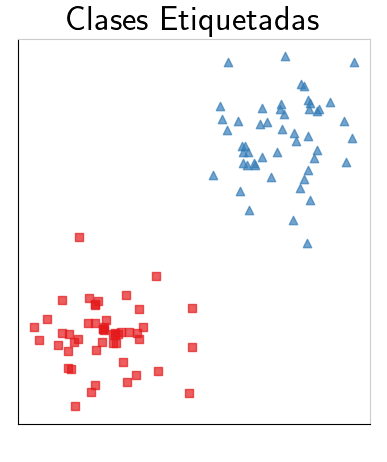
\includegraphics[width=0.8\linewidth]{imagenes/chapter2/BeforeSVMExample.png} 
  \tikz[remember picture]\node[inner sep=0pt,outer sep=0pt] (a) {}; 
    \end{subfigure}
    \begin{subfigure}{.3\textwidth} 
  \centering
  \tikz[remember picture]\node[inner sep=0pt,outer sep=0pt] (b) {}; 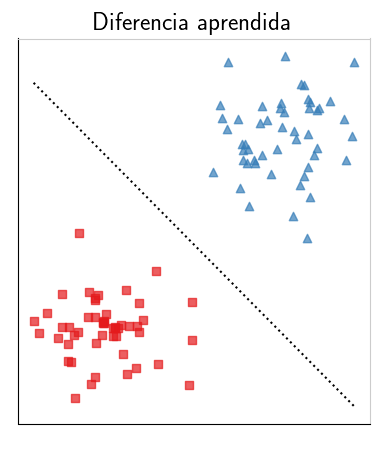
\includegraphics[width=0.8\linewidth]{imagenes/chapter2/AfterSVMExample.png}
    \end{subfigure}
  \tikz[remember picture,overlay]\draw[line width=1pt,-stealth,black] ([xshift=2mm,yshift=2cm]a.east) -- ([xshift=-2mm, yshift=2cm]b.west)node[midway,above,text=black,font=\LARGE\bfseries\sffamily] {};
  \caption[Ejemplo de aprendizaje supervisado.]{
  Ejemplo de aprendizaje supervisado. Vemos como a partir de un conjunto de clases etiquetadas aprendemos un hiper plano que 
  las separa. 
  }
  \label{fig:SupervisedExample}
\end{figure}
\begin{figure}[htp]
  \centering
    \begin{subfigure}{.3\textwidth}
  \centering
  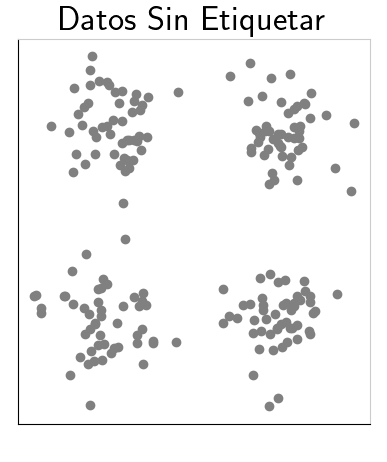
\includegraphics[width=0.8\linewidth]{imagenes/chapter2/BeforeClusteringExample.png} 
  \tikz[remember picture]\node[inner sep=0pt,outer sep=0pt] (c) {}; 
    \end{subfigure}
    \begin{subfigure}{.3\textwidth} 
  \centering
  \tikz[remember picture]\node[inner sep=0pt,outer sep=0pt] (d) {}; 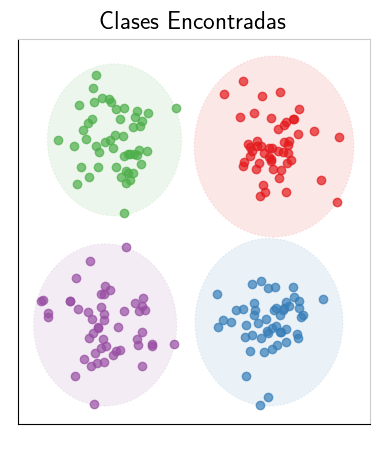
\includegraphics[width=0.8\linewidth]{imagenes/chapter2/AfterClusteringExample.png}
    \end{subfigure}
  \tikz[remember picture,overlay]\draw[line width=1pt,-stealth,black] ([xshift=2mm,yshift=2cm]c.east) -- ([xshift=-2mm, yshift=2cm]d.west)node[midway,above,text=black,font=\LARGE\bfseries\sffamily] {};

  \caption[Ejemplo de aprendizaje no supervisado.]{
  Ejemplo de aprendizaje no supervisado. Dado un conjunto de puntos aprendemos un conjunto de clases 
  a partir de los patrones.
}
  \label{fig:UnsupervisedExample}
\end{figure}

\subsection{Aprendizaje Profundo}
En el aprendizaje profundo o \emph{Deep Learning} (\emph{DL}), 
a diferencia de los modelos anteriores donde tenemos un conjunto de variables 
extraídas por un humano experto, las características sobre la cual inferimos 
son obtenidas por el propio modelo automáticamente~\cite{DeepLMITPress, DeepLearningNature, DeepLearningInNN}.
En términos generales, la extracción automática de características suele 
desempeñar mejores resultados en contra de las características manuales.

La mayoría de los modelos de DL son basados en múltiples capas jerárquicas de 
procesado de datos. Las más conocidas son las redes neuronales (ANN, por sus siglas 
en inglés), modelo bioinspirado que simula el funcionamiento de las neuronas del cerebro
humano (abstracción simplificada)~\cite{ANNForPattern,ANNCambridge}. 

A alto nivel, el funcionamiento de una red neuronal implica tres etapas principales: 
entrada, procesamiento y salida. En la etapa de entrada, se proporciona a la red 
neuronal un conjunto de datos o características que representan la información 
que se desea analizar o procesar. Estos datos de entrada se propagan a través 
de la red neuronal (\emph{feedforward}). En la etapa de procesamiento, las neuronas reciben las entradas 
y realizan cálculos utilizando pesos y funciones de activación. Los pesos representan 
la importancia relativa de las diferentes entradas en el cálculo, y las funciones 
de activación determinan la salida de una neurona en función de su entrada. A medida que los datos se propagan a través de la red neuronal, las capas intermedias 
procesan y combinan las entradas, extrayendo características relevantes y creando 
representaciones internas cada vez más abstractas. Esto permite que la red neuronal aprenda y 
descubra patrones en los datos. Finalmente, en la etapa de salida, la red neuronal 
produce una respuesta o predicción basada en las características extraídas. 
Esto puede ser la clasificación de una imagen, la predicción de un valor numérico o 
cualquier otro resultado deseado. En esta última etapa se calcula el error de 
predicción respecto a la salida deseada con la función de pérdida y se ajusta 
los pesos respectivamente.

El aprendizaje de una red neuronal se logra mediante un proceso llamado entrenamiento.
Donde de forma iterativa repetimos el proceso descrito anteriormente varias veces 
con distintos ejemplos. El conjunto de datos es muy relevante para el correcto 
aprendizaje. Debe de ser representativo, extenso y limpio de anormalidades ya que 
estaremos extrayendo características y relevancias a partir de ellos.

En definitiva, una red neuronal es en esencia una serie de ajustes de parámetros para lograr el resultado deseado. 
Estos incluyen ajuste de los pesos y sesgos iniciales, selección de las funciones de activación, 
como las más utilizadas sigmoide o ReLU, de una función de pérdida y un optimizador, 
encargado de determinar como ajustar los pesos según el error obtenido en cada fase del entrenamiento.
No obstante, existe un fenómeno denominado sobreentrenamiento o \emph{overfitting}. 
Ocurre cuando hay un sobreajuste de los parámetros
hacia los datos de entrenamiento, disminuyendo la capacidad de generalización del modelo. 
Informalmente, es como decir que el modelo ha memorizado los resultados y, por ello, 
con datos nunca vistos posee errores substancialmente altos. Para lidiar con estos 
problemas se deben elegir también formas de regularización del modelo, es decir, 
restricciones sobre el entrenamiento para evitar el sobre ajuste. 

\begin{figure}[htp]
  \centering
  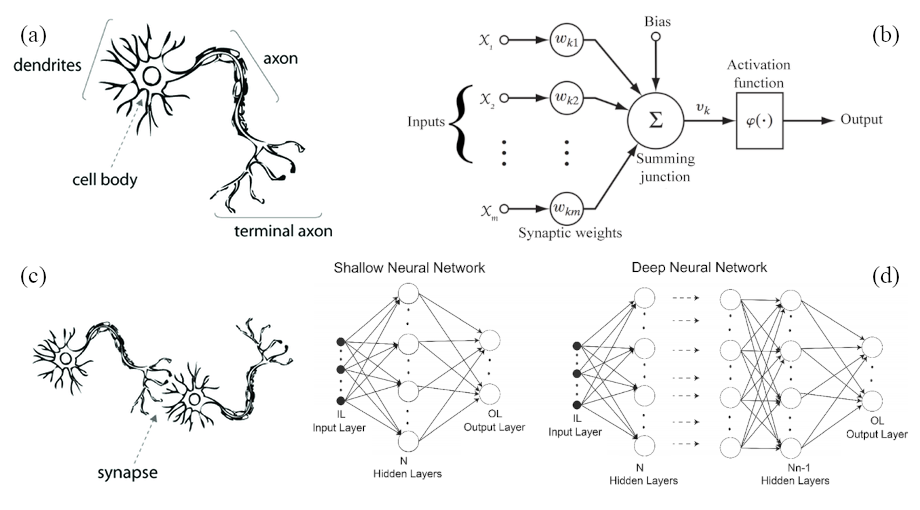
\includegraphics[width=\textwidth]{imagenes/chapter2/ANNVisualization.png}
  \caption[Ejemplo gráfico de una red neuronal.]
  {Ejemplo gráfico de una red neuronal~\cite{NeuronImages, NeuronSimilarity,ShallowAndDeepNN}. 
    (a) y (b) muestran una neurona biológica y una artificial, respectivamente. 
    (c) visualiza la sinapsis (o proceso mediante el cual las neuronas se comunican 
    entre sí para transmitir información). (d) muestra dos redes neuronales artificiales: 
    a la izquierda, una red neuronal superficial (\emph{shallow}), con una única 
    capa oculta; a la derecha, una red neuronal profunda (\emph{deep}), con múltiples capas ocultas.
  }
  \label{fig:ANNVisualization}
\end{figure}

\subsubsection{Redes Convolucionales} 
Las redes convolucionales o \emph{convolutional neural network} (CNN)~\cite{ConvolutionalZipCode, ConvolutionInRadiology}
son un tipo de arquitectura de redes neuronales diseñadas 
específicamente para el procesamiento de datos estructurados en forma de matrices, como imágenes.
Se ha descubierto que son aplicables para el procesado de texto, sonidos y, recientemente,
a superficies tridimensionales.
Utilizan capas convolucionales que aplican filtros a regiones locales de la entrada 
para extraer características relevantes. En la Figura \ref{fig:RadiographyConvolutionExample}
podemos ver un ejemplo de esquema jerárquico de extracción de características para el 
diagnóstico médico a partir de una radiografía. Se puede observar 
que, a diferencia de una ANN, existen dos capas adicionales: capas convolucionales 
y capas de \emph{pooling}.

\begin{figure}[htp]
  \centering
  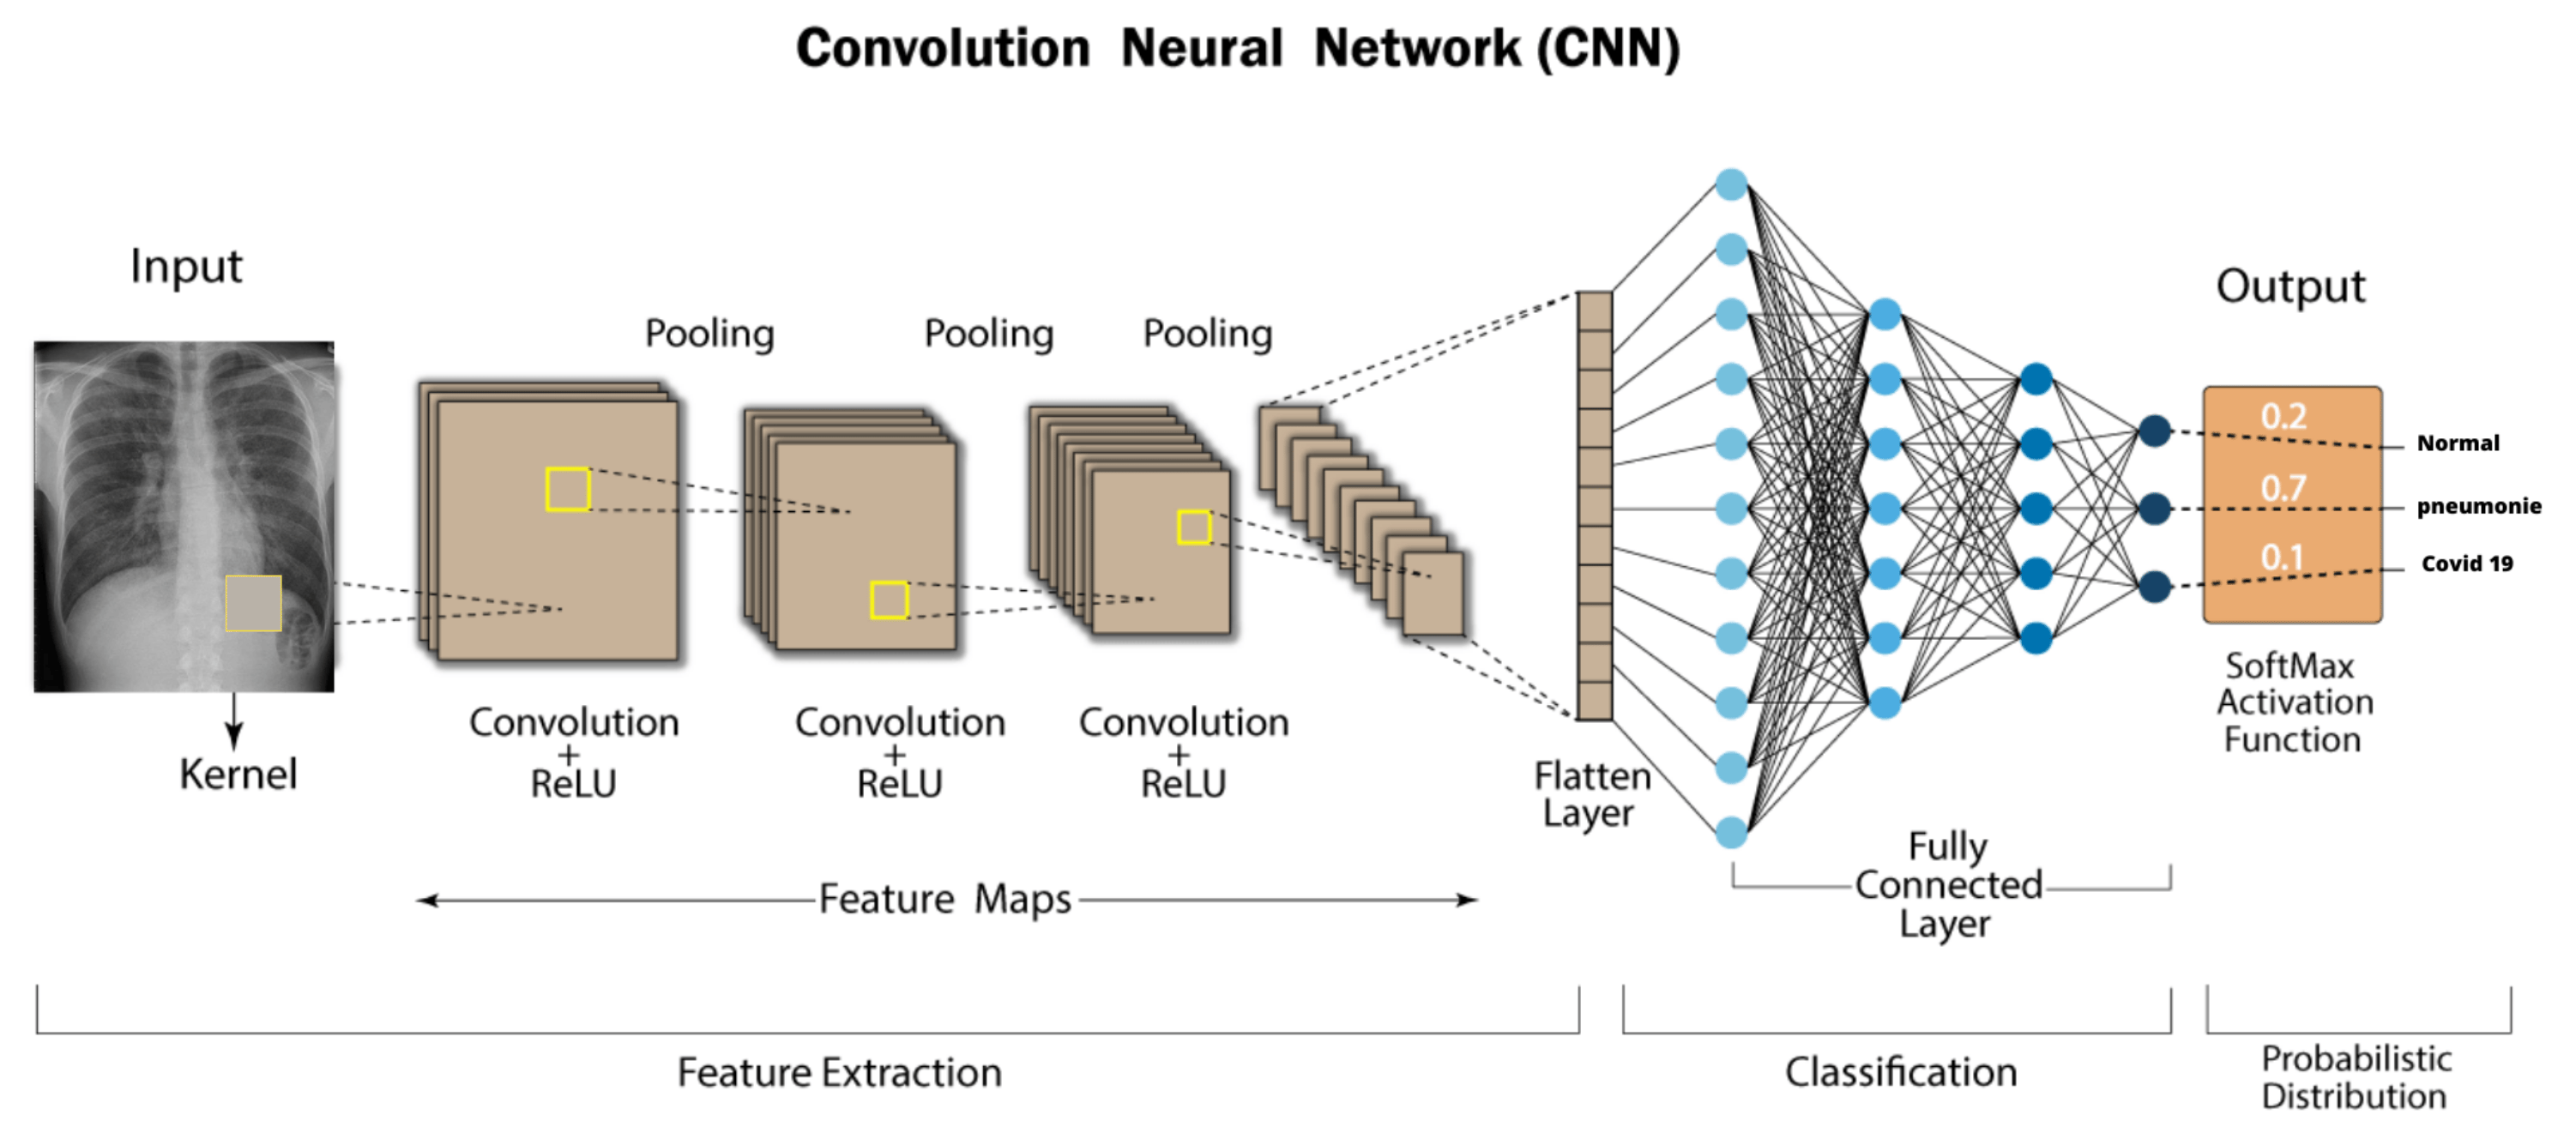
\includegraphics[width=\textwidth]{imagenes/chapter2/RadiographyConvolutionExample.png}
  \caption[Ejemplo de red convolucional para imágenes médicas]{
    Red neuronal convolucional (CNN) aplicada a un problema de clasificación de imágenes biomédicas~\cite{RadiographyConvolutionExample}.
    Se pueden identificar los principales bloques constitutivos de una CNN: capa convolucional, 
    capa de pooling, función de activación, y capa totalmente conectada.
  }
  \label{fig:RadiographyConvolutionExample}
\end{figure}

\subsubsection{Capas convolucionales}
Para simplificar la explicación, la realizaremos sobre imágenes 2D. 
Una capa convolucional es encargada de realizar la operación de convolución sobre 
los datos de entrada. 
La convolución se refiere a una operación matemática que combina dos funciones para crear una tercera función.
En este caso, se aplica una operación de convolución 
entre una matriz de entrada (como una imagen) y un filtro (\emph{kernel}).
La operación de convolución implica deslizar el filtro sobre la matriz de entrada, 
multiplicando los elementos coincidentes y sumándolos para obtener un único valor 
en la matriz de salida, conocida como mapa de características. 
Este proceso se repite en diferentes ubicaciones de la matriz de 
entrada para generar el mapa de características completo. En la Figura 
\ref{fig:ConvolutionalRepresentation} vemos una operación sobre la ubicación 
inicial de la imagen, esquina superior izquierda. 
La elección del siguiente trozo 
o \emph{patch} de la imagen suele venir determinado por el paso o \emph{stride}.
Habitualmente se utiliza un \emph{stride} de 1. Es decir, elegimos la matriz 
adyacente con distancia horizontal igual a 1 hasta llegar al final de esa fila 
y luego nos desplazamos 1 hacia abajo. 
Por medio de este proceso, la red es capaz de
capturar dependencias temporales y espaciales en los datos con la aplicación
de los filtros correspondientes.

Podemos observar en la Figura \ref{fig:ConvolutionalRepresentation} que aplicar directamente 
el operador de convolución a una imagen resulta en una reducción del tamaño del mapa 
de activación debido a la naturaleza del operador. 
Sin embargo, esto no siempre es deseable. 
Para abordar este problema, se puede agregar relleno o \emph{padding} a la imagen 
de entrada utilizando información existente en la misma. 
Esto garantiza que el mapa de activación tenga la misma dimensionalidad que 
la imagen original. Además, es posible reducir aún más la salida ajustando 
los saltos o \emph{strides} del filtro de convolución mientras se recorre la imagen.

\begin{figure}[htp]
  \begin{center}
    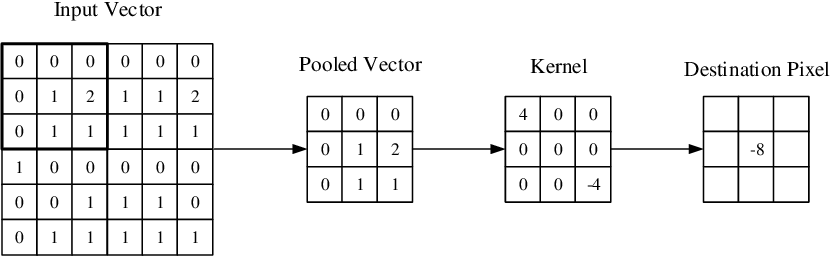
\includegraphics[width=0.95\textwidth]{imagenes/chapter2/ConvolutionalRepresentation.png}
  \end{center}
  \caption[Representación visual de la operación de convolución]{Representación visual de la operación de convolución sobre una imagen, extraída de~\cite{ConvolutionalRepresentation}.
  }
  \label{fig:ConvolutionalRepresentation}
\end{figure}

\subsubsection{Capa de pooling} 
El propósito principal de las capas de \emph{pooling} es reducir la cantidad de parámetros 
y la complejidad computacional de la red, al tiempo que conservan las características 
más relevantes. Además, el \emph{pooling} puede ayudar a hacer que la representación sea 
invariante a pequeñas variaciones en la posición o el tamaño de los objetos en la 
imagen, lo que mejora la capacidad de generalización del modelo.

En la Figura \ref{fig:PoolingExample} vemos un operador de \emph{pooling} común,
el operador de valor máximo. También es habitual el uso del operador de valor medio y
valor mínimo.
El \emph{pooling}, al igual que la convolución, posee un filtro o ventana que recorre
los datos dado un salto o \emph{stride} al moverse por los mismos.

Las capas convolucionales y de \emph{pooling} trabajan en conjunto para procesar y extraer 
características. 
Dependiendo de la complejidad del problema, se puede ajustar el número de estas.

\begin{figure}[htp]
  \begin{center}
    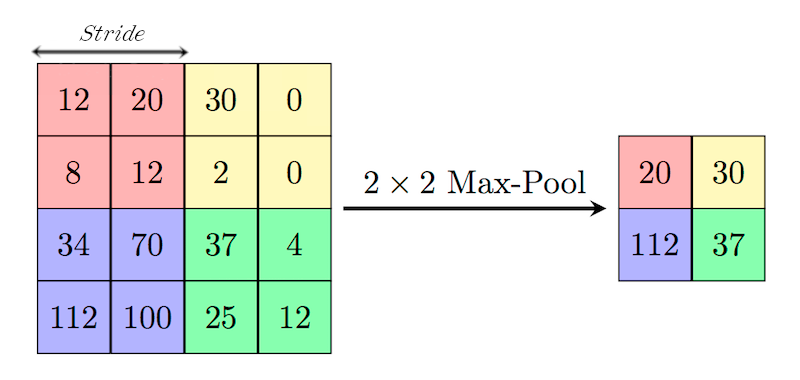
\includegraphics[width=0.65\textwidth]{imagenes/chapter2/MaxpoolSample.png}
  \end{center}

  \caption{
    Ejemplo de operación de \emph{max-pooling} con \emph{stride} a 2x2.
  }
  \label{fig:PoolingExample}
\end{figure}

\subsubsection{Capas totalmente conectadas}
Las capas totalmente conectadas o \emph{fully connected}, también llamadas 
capas densas o \emph{dense}, son aquellas en las que todas sus neuronas 
están conectadas con todas las neuronas de la capa anterior y de la
siguiente. Si bien existen modelos totalmente convolucionales, resulta común
que las CNNs incluyan capas totalmente conectadas al final de la arquitectura.
Estas capas forman una ANN clásica.
La salida de la última capa densa, siendo la salida de la red entera, es donde
se evaluará la función de pérdida elegida y, al igual que en una red neuronal
clásica, se utilizará este valor para ajustar los pesos.

\subsubsection{Aplicadas a Videos} 
\label{sec:VideoCNN}
Las redes convolucionales se pueden llegar a aplicar incluso a videos. 
Para ello, se puede utilizar una variante de las redes convolucionales llamada 
redes convolucionales 3D (3D CNNs) o redes convolucionales espaciotemporales. 
Estas redes están diseñadas específicamente para capturar tanto las características 
espaciales como las temporales presentes en los vídeos.

La principal diferencia entre una red convolucional tradicional y una 3D CNN es 
la adición de una dimensión temporal en las operaciones de convolución. 
En lugar de considerar solo imágenes individuales, se toman secuencias de imágenes 
(\emph{frames}) para capturar la información temporal.

En este TFG se explora el uso de una 3D CNN capaz de analizar vídeos que pertenece 
a la familia que se conoce como \emph{SlowFast networks}~\cite{SlowFastNetworks}. Están basadas en dos caminos 
de entrada de datos. Un conjunto de \emph{frames} espaciados en el tiempo, 
\emph{slow path}, para obtener información espacial y otro con todos ellos, \emph{fast path}, 
para obtener información de movimiento (véase Figura \ref{fig:SlowFastPathways}). 

\begin{figure}[htp]
  \begin{center}
    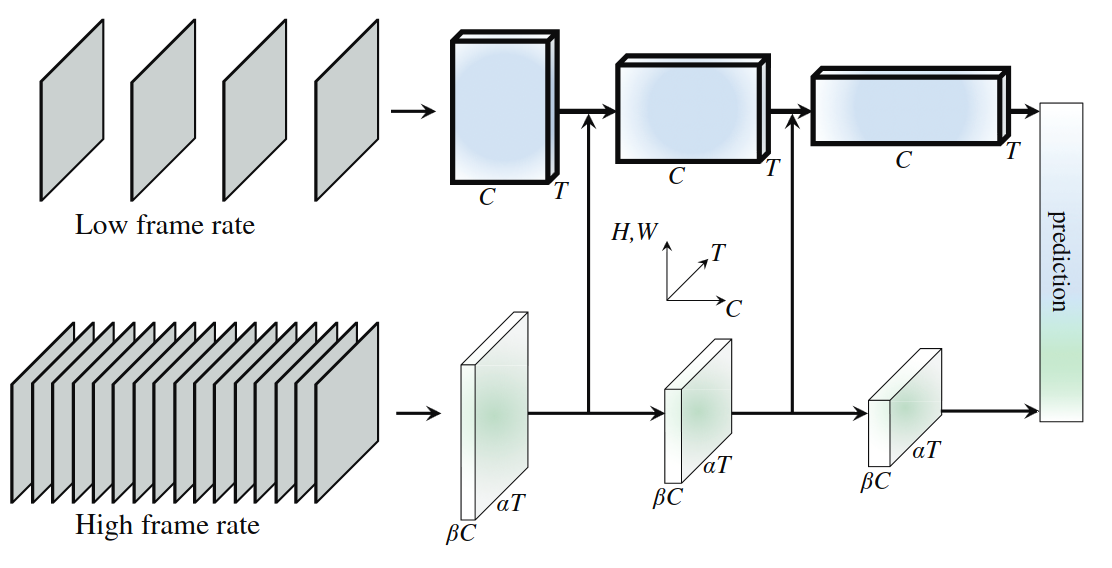
\includegraphics[width=0.5\textwidth]{imagenes/chapter2/SlowFastPathways.png}
  \end{center}
  \caption[Red convolucional espaciotemporal \emph{SlowFast}.]{Ejemplo extraído de~\cite{SlowFastNetworks} para ilustrar la distinción 
  entre la extracción espacial del camino ``\emph{slow path}'' (camino superior) y 
  de movimiento con el camino ``\emph{fast path}'' (camino inferior).}
  \label{fig:SlowFastPathways}
\end{figure}

\subsubsection{Aplicadas a nubes de puntos}

De forma similar al caso de los videos, actualmente existen modelos de 3D CNNs 
capaces de procesar nubes de puntos al añadir una dimensión más que representa 
la profundidad de los píxeles.  Sin embargo, la complejidad de diseño y tiempo de cómputo para 
estos modelos 3D crece enormemente. Esto es debido a que, habitualmente, las nubes de puntos 
están formadas por puntos dispersos en el espacio, en lo que denominamos datos 
sin estructura ni orden propio, y debemos mapear una operación 
de convolución que está basada en operaciones sobre datos ordenados y estructurados. 

Aunque cada vez hay más métodos que se aplican directamente sobre la nube de puntos 
desde la publicación de \emph{PointNet}~\cite{PointNet}, habitualmente se 
intenta estructurar la información de las nubes de puntos mediante lo que 
denominamos vóxeles~\cite{VoxelizationExample}. 
La voxelización es el proceso de transformar una nube de puntos u otra representación 
tridimensional en una estructura discreta conocida como volumen voxelizado. 
Esto implica dividir el espacio tridimensional en una cuadrícula de vóxeles y asignar 
valores a cada vóxel según la información contenida en los datos originales. 
La voxelización proporciona una representación estructurada y discreta que permite 
el uso de técnicas específicas para volúmenes y facilita el procesamiento y análisis 
de datos 3D.

\begin{figure}[htp]
  \centering
  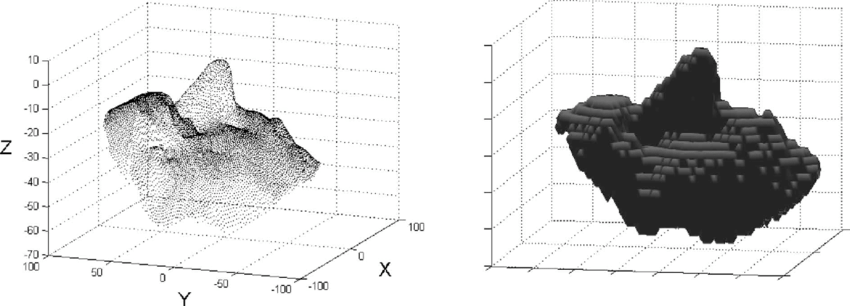
\includegraphics[width=0.80\textwidth]{imagenes/chapter2/VoxelizationExample.png}
  \caption[Ejemplo gráfico sobre voxelización.]{Ejemplo extraído de~\cite{VoxelizationExample} que demuestra el resultado 
  de transformar una nube de puntos sin estructura en una cuadrícula voxelizada.}
  \label{fig:VoxelizationExample}
\end{figure}

\subsection{Ensemble de modelos de Deep Learning}
Un \emph{ensemble}, en el contexto del aprendizaje automático, es una técnica que 
combina múltiples modelos de aprendizaje para mejorar la precisión y el rendimiento 
general de las predicciones. En lugar de depender de un único modelo, 
se crean múltiples modelos y se combinan sus predicciones para obtener un resultado 
final más robusto y preciso~\cite{IAModernApproach, DataMiningHandbook, MedicalEnsembleExample}.

La idea fundamental detrás de los \emph{ensembles} es que los diferentes modelos pueden 
tener fortalezas y debilidades diferentes, y al combinar sus predicciones, se 
puede obtener una mejor generalización y un mayor rendimiento en una variedad de 
situaciones. Para construir un \emph{ensemble} se suele utilizar un conjunto 
de técnicas que se describirán a continuación. 

El \emph{bagging} consiste en generar múltiples conjuntos de datos de entrenamiento 
mediante muestreo con reemplazo, entrenando un modelo en cada conjunto y 
promediando o ponderando sus predicciones. 
En el \emph{boosting}, los modelos se construyen secuencialmente, corrigiendo los errores 
del modelo anterior, y se combinan para formar un modelo más fuerte. 
La aumentación de datos consiste en ampliar el conjunto de entrenamiento para
mejorar la capacidad de generalización del modelo y reducir el sobreajuste por 
medio de transformaciones sobre los datos como la rotación y ampliación, 
se podría usar como paso en el proceso de \emph{bagging}.
Los \emph{random forests} combinan \emph{bagging} y árboles de decisión, 
generando múltiples árboles utilizando diferentes subconjuntos de datos y características. 
Las predicciones de los árboles individuales se combinan para obtener la predicción final.
Por último, el \emph{stacking} entrena múltiples modelos base y utiliza un meta-modelo 
para combinar sus predicciones. 
Cada estrategia tiene sus beneficios y consecuencias.

El presente TFG evalúa el uso de un meta-modelo para la estimación de calidad de 
las imágenes médicas 3D sin referencia.

\begin{figure}[htp]
  \centering
  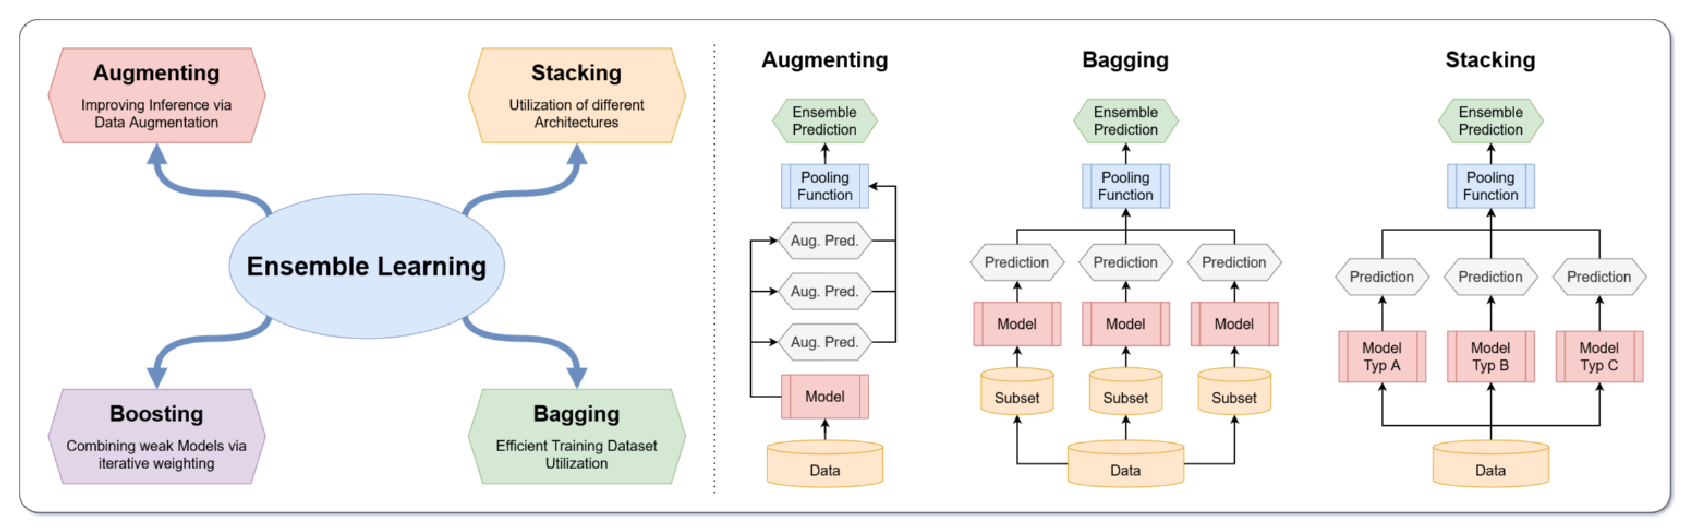
\includegraphics[width=\textwidth]{imagenes/chapter2/EnsembleExample.png}
  \caption[Representación de métodos de \emph{ensemble}.]{Representación de métodos de \emph{ensemble}~\cite{MedicalEnsembleExample}.
    A la izquierda vemos una definición general de los distintos tipos de \emph{ensemble}. A la derecha, el primer esquema es sobre 
    aumentación de datos (un conjunto de datos y un modelo que se entrena con varias ejemplos alterados o no). El siguiente 
    esquema representa \emph{bagging} (el mismo modelo entrenado con distintos subconjuntos de datos). 
    Por último, observamos el empleo de \emph{stacking} (distintos modelos entrenados con el mismo conjunto de datos).
  }
  \label{fig:EnsembleExample}
\end{figure}

\section{Imágenes médicas y distorsiones}
\label{sec:Distorsiones}
Las tomografías computarizadas son un tipo de técnica de imagen médica 
que utiliza rayos X para obtener imágenes detalladas del interior del cuerpo. 
Durante una tomografía computarizada, el paciente se coloca en una mesa que se 
mueve a través de un anillo en forma de donut llamado \emph{gantry}. Dentro del \emph{gantry},
se encuentra un tubo de rayos X que gira alrededor del paciente, emitiendo haces 
de rayos X en forma de abanico.
Los detectores ubicados en el lado opuesto del \emph{gantry} registran la cantidad de 
rayos X que atraviesan el cuerpo del paciente. Estos datos se recopilan en 
múltiples ángulos y se utilizan para reconstruir imágenes transversales del cuerpo. 

\begin{figure}[htp]
  \begin{subfigure}{2\textwidth}
  \hspace{1cm}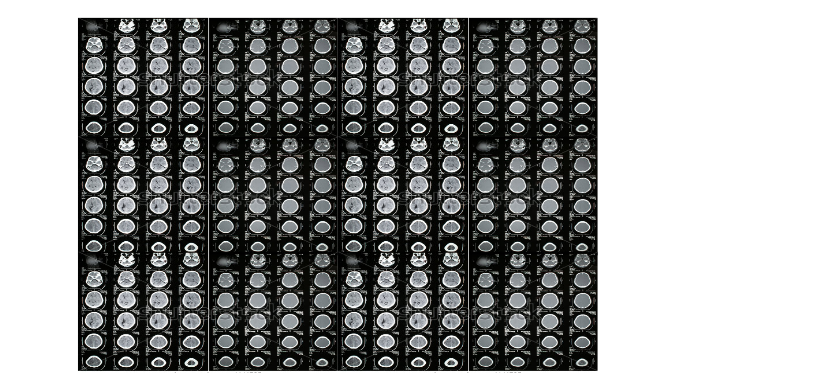
\includegraphics[width=0.5\textwidth]{imagenes/chapter2/CTDir.png}
  \end{subfigure}
  \begin{subfigure}{2\textwidth}
  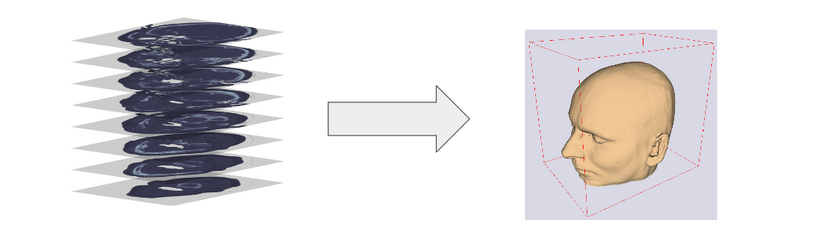
\includegraphics[width=0.5\textwidth]{imagenes/chapter2/CT2Volume.png}
  \end{subfigure}
  \caption[Ejemplo de tomografía computarizada y modelo 3D.]{Ejemplo de tomografía computarizada y modelo 3D~\cite{CT2Volume}.}
  \label{fig:CT2Volume}
\end{figure}

El número de imágenes en una tomografía computarizada se selecciona en función 
de varios factores, como el área del cuerpo que se está examinando, el propósito 
clínico de la exploración y las preferencias del radiólogo o médico que interpreta 
las imágenes. Ajustar el número de imágenes puede influir en el tiempo de adquisición, 
la cantidad de radiación utilizada y la cantidad de información detallada que se 
obtiene de la exploración. Afecta directamente a la calidad del modelo 3D generado 
al final, ya que el número de cortes es la tercera dimensión que relaciona las imágenes 
(profundidad).

Sobre todo nos centraremos en las distorsiones geométricas que ocurren en la 
generación volumétrica de la imagen. La generación del volumen consiste en 
disponer de un conjunto segmentado\footnote{
La segmentación se refiere al proceso de dividir una imagen o conjunto de datos en regiones o componentes más pequeños. 
Ejemplo, en una foto del bosque, segmentamos los árboles para distinguirlos del suelo.
} en todas las capas de las imágenes. A continuación usando el conjunto segmentado 
unificamos las coordenadas de los puntos por medio de intersecciones entre rayos 
proyectados sobre las imágenes (\emph{ray casting}, véase Figura \ref{fig:CT2Volume}).

% \begin{figure}[htp]
%   \centering 
%   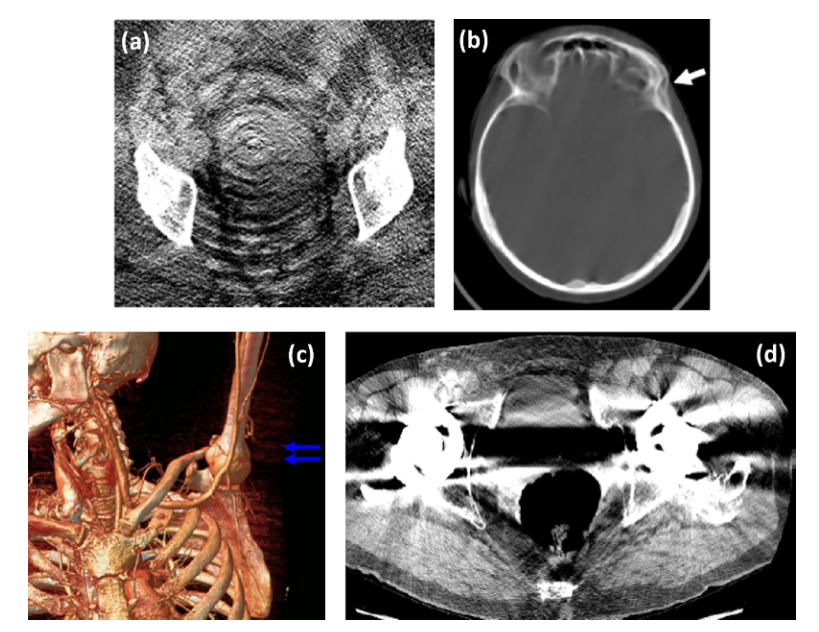
\includegraphics[width=\textwidth]{imagenes/chapter2/DicomDistortionsExample.png}
%   \caption[Ejemplo de artefactos sobre imágenes DICOM.]{Ejemplo de artefactos sobre imágenes DICOM~\cite{DicomDistortionsExample}: 
%   (a) un artefacto de anillo, (b) un difuminado provocado por movimiento, 
%   (c) artefactos producidos por interpolación helicoidal, (d) artefactos de iluminación y dispersión del haz.  }
%   \label{fig:DicomDistortionsExample}
% \end{figure}

Dentro de las causas de las distorsiones geométricas sobre los volúmenes 
3D están el difuminado por movimiento, errores de contraste (dificultad al segmentar),
artefactos luminosos y problemas de interpolación o ruido al generar la proyección. 


